% questions.tex —— 2004 年·普通高等学校招生考试·湖北卷·理科 · 题目内容片段（无答案）
% 由 tools/generate_projects.py 依来源总账自 2004/2004_数学真题_湖北理科_试题.md 生成，勿手改（改源 MD 后重跑）

\gkpart{一、选择题：本大题共 12 小题，每小题 5 分，共 60 分．在每小题给出的四个选项中，只有一项是符合题目要求的．}

\begin{question}
\gkti{1}与直线 $2x - y + 4 = 0$ 平行的抛物线 $y = x^2$ 的切线方程是\mbox{（　　）}

\begin{gkopts}(4)
\task A．$2x - y + 3 = 0$
\task B．$2x - y - 3 = 0$
\task C．$2x - y + 1 = 0$
\task D．$2x - y - 1 = 0$
\end{gkopts}

\end{question}
\begin{question}
\gkti{2}复数 $\dfrac{(-1 + \sqrt{3}\mathrm{i})^5}{1 + \sqrt{3}\mathrm{i}}$ 的值是\mbox{（　　）}

\begin{gkopts}(1)
\task A．$-16$
\task B．$16$
\task C．$-\dfrac{1}{4}$
\task D．$\dfrac{1}{4} - \dfrac{\sqrt{3}}{4}\mathrm{i}$
\end{gkopts}

\end{question}
\begin{question}
\gkti{3}已知 $f\left(\dfrac{1 - x}{1 + x}\right) = \dfrac{1 - x^2}{1 + x^2}$，则 $f(x)$ 的解析式可取为\mbox{（　　）}

\begin{gkopts}(2)
\task A．$\dfrac{x}{1 + x^2}$
\task B．$-\dfrac{2x}{1 + x^2}$
\task C．$\dfrac{2x}{1 + x^2}$
\task D．$-\dfrac{x}{1 + x^2}$
\end{gkopts}

\end{question}
\begin{question}
\gkti{4}已知 $\vec{a}, \vec{b}, \vec{c}$ 为非零的平面向量．甲：$\vec{a} \cdot \vec{b} = \vec{a} \cdot \vec{c}$，乙：$\vec{b} = \vec{c}$，则\mbox{（　　）}

\begin{gkopts}(2)
\task A．甲是乙的充分条件但不是必要条件
\task B．甲是乙的必要条件但不是充分条件
\task C．甲是乙的充要条件
\task D．甲既不是乙的充分条件也不是乙的必要条件
\end{gkopts}

\end{question}
\begin{question}
\gkti{5}若 $\dfrac{1}{a} < \dfrac{1}{b} < 0$，则下列不等式① $a + b < ab$；② $|a| > |b|$；③ $a < b$；④ $\dfrac{b}{a} + \dfrac{a}{b} > 2$ 中，正确的不等式有\mbox{（　　）}

\begin{gkopts}(4)
\task A．$1$ 个
\task B．$2$ 个
\task C．$3$ 个
\task D．$4$ 个
\end{gkopts}

\end{question}
\begin{question}
\gkti{6}已知椭圆 $\dfrac{x^2}{16} + \dfrac{y^2}{9} = 1$ 的左、右焦点分别为 $F_1$、$F_2$，点 $P$ 在椭圆上，若 $P$、$F_1$、$F_2$ 是一个直角三角形的三个顶点，则点 $P$ 到 $x$ 轴的距离为\mbox{（　　）}

\begin{gkopts}(2)
\task A．$\dfrac{9}{5}$
\task B．$3$
\task C．$\dfrac{9\sqrt{7}}{7}$
\task D．$\dfrac{9}{4}$
\end{gkopts}

\end{question}
\begin{question}
\gkti{7}函数 $f(x) = a^x + \log_a (x + 1)$ 在 $[0, 1]$ 上的最大值与最小值之和为 $a$，则 $a$ 的值为\mbox{（　　）}

\begin{gkopts}(4)
\task A．$\dfrac{1}{4}$
\task B．$\dfrac{1}{2}$
\task C．$2$
\task D．$4$
\end{gkopts}

\end{question}
\begin{question}
\gkti{8}设数列 $\{a_n\}$ 的前 $n$ 项和 $S_n = a\left[2 - \left(\dfrac{1}{2}\right)^{n-1}\right] - b\left[2 - (n + 1)\left(\dfrac{1}{2}\right)^{n-1}\right]$（$n = 1, 2, \cdots$），其中 $a$、$b$ 是非零常数．则存在数列 $\{x_n\}$、$\{y_n\}$ 使得\mbox{（　　）}

\begin{gkopts}(1)
\task A．$a_n = x_n + y_n$，其中 $\{x_n\}$ 为等差数列，$\{y_n\}$ 为等比数列
\task B．$a_n = x_n + y_n$，其中 $\{x_n\}$ 和 $\{y_n\}$ 都为等差数列
\task C．$a_n = x_n \cdot y_n$，其中 $\{x_n\}$ 为等差数列，$\{y_n\}$ 为等比数列
\task D．$a_n = x_n \cdot y_n$，其中 $\{x_n\}$ 和 $\{y_n\}$ 都为等比数列
\end{gkopts}

\end{question}
\begin{question}
\gkti{9}函数 $f(x) = ax^3 + x + 1$ 有极值的充要条件是\mbox{（　　）}

\begin{gkopts}(4)
\task A．$a > 0$
\task B．$a \geqslant 0$
\task C．$a < 0$
\task D．$a \leqslant 0$
\end{gkopts}

\end{question}
\begin{question}
\gkti{10}设集合 $P = \{m \mid -1 < m < 0\}$，$Q = \{m \in \mathbf{R} \mid mx^2 + 4mx - 4 < 0$ 对任意实数 $x$ 恒成立$\}$，则下列关系中成立的是\mbox{（　　）}

\begin{gkopts}(2)
\task A．$P \subsetneqq Q$
\task B．$Q \subsetneqq P$
\task C．$P = Q$
\task D．$P \cap Q = \varnothing$
\end{gkopts}

\end{question}
\begin{question}
\gkti{11}已知平面 $\alpha$ 与 $\beta$ 所成的二面角为 $80^\circ$，$P$ 为 $\alpha, \beta$ 外一定点，过点 $P$ 的一条直线与 $\alpha, \beta$ 所成的角都是 $30^\circ$，则这样的直线有且仅有\mbox{（　　）}

\begin{gkopts}(4)
\task A．$1$ 条
\task B．$2$ 条
\task C．$3$ 条
\task D．$4$ 条
\end{gkopts}

\end{question}
\begin{question}
\gkti{12}设 $y = f(t)$ 是某港口水的深度 $y$（米）关于时间 $t$（时）的函数，其中 $0 \leqslant t \leqslant 24$，下表是该港口某一天从 $0$ 时至 $24$ 时记录的时间 $t$ 与水深 $y$ 的关系：

\begin{center}
\begingroup\setlength{\tabcolsep}{4pt}
\begin{tabular}{cccccccccc}
\toprule
$t$ & $0$ & $3$ & $6$ & $9$ & $12$ & $15$ & $18$ & $21$ & $24$ \\
\midrule
$y$ & $12$ & $15.1$ & $12.1$ & $9.1$ & $11.9$ & $14.9$ & $11.9$ & $8.9$ & $12.1$ \\
\bottomrule
\end{tabular}
\endgroup
\end{center}

经长期观察，函数 $y = f(t)$ 的图象可以近似地看成函数 $y = k + A\sin(\omega t + \varphi)$ 的图象．下面的函数中，最能近似表示表中数据间对应关系的函数是\mbox{（　　）}

\begin{gkopts}(1)
\task A．$y = 12 + 3\sin\dfrac{\pi}{6}t, t \in [0, 24]$
\task B．$y = 12 + 3\sin\left(\dfrac{\pi}{6}t + \pi\right), t \in [0, 24]$
\task C．$y = 12 + 3\sin\dfrac{\pi}{12}t, t \in [0, 24]$
\task D．$y = 12 + 3\sin\left(\dfrac{\pi}{12}t + \dfrac{\pi}{2}\right), t \in [0, 24]$
\end{gkopts}

\end{question}
\gkpart{二、填空题：本大题共 4 小题，每小题 4 分，共 16 分．把答案填在横线上．}

\begin{question}
\gkti{13}设随机变量 $\xi$ 的概率分布为 $P(\xi = k) = \dfrac{a}{5^k}$，$a$ 为常数，$k = 1, 2, \cdots$，则 $a =$ \gkblank{}．

\end{question}
\begin{question}
\gkti{14}将标号为 $1, 2, \cdots, 10$ 的 $10$ 个球放入标号为 $1, 2, \cdots, 10$ 的 $10$ 个盒子内，每个盒内放一个球，则恰好有 $3$ 个球的标号与其所在盒子的标号不一致的放入方法共有 \gkblank{} 种．（以数字作答）

\end{question}
\begin{question}
\gkti{15}设 $A$、$B$ 为两个集合．下列四个命题：

① $A \not\subseteq B \iff \text{\text{对任意} } x \in A, \text{\text{有} } x \notin B$；

② $A \not\subseteq B \iff A \cap B = \varnothing$；

③ $A \not\subseteq B \iff A \not\supseteq B$；

④ $A \not\subseteq B \iff \text{\text{存在} } x \in A, \text{\text{使得} } x \notin B$．

其中真命题的序号是 \gkblank{}．（把符合要求的命题序号都填上）

\end{question}
\begin{question}
\gkti{16}某日中午 12 时整，甲船自 $A$ 处以 $16\text{ km/h}$ 的速度向正东行驶，乙船自 $A$ 的正北 $18\text{ km}$ 处以 $24\text{ km/h}$ 的速度向正南行驶，则当日 12 时 30 分时两船之距离对时间的变化率是 \gkblank{} $\text{km/h}$．

\end{question}
\gkpart{三、解答题：本大题共 6 小题，共 74 分．解答应写出文字说明，证明过程或演算步骤．}

\begin{question}
\gkti{17}已知 $6\sin^2\alpha + \sin\alpha\cos\alpha - 2\cos^2\alpha = 0$，$\alpha \in \left[\dfrac{\pi}{2}, \pi\right]$，求 $\sin\left(2\alpha + \dfrac{\pi}{3}\right)$ 的值．

\Needspace{0.4\textheight}
\end{question}
\begin{question}
\gkti{18}如图，在棱长为 $1$ 的正方体 $ABCD - A_1B_1C_1D_1$ 中，点 $E$ 是棱 $BC$ 的中点，点 $F$ 是棱 $CD$ 上的动点．

（1）试确定点 $F$ 的位置，使得 $D_1E \perp \text{\text{平面} } AB_1F$；

（2）当 $D_1E \perp \text{\text{平面} } AB_1F$ 时，求二面角 $C_1 - EF - A$ 的大小．（结果用反三角函数值表示）
\nopagebreak[4]
\begin{center}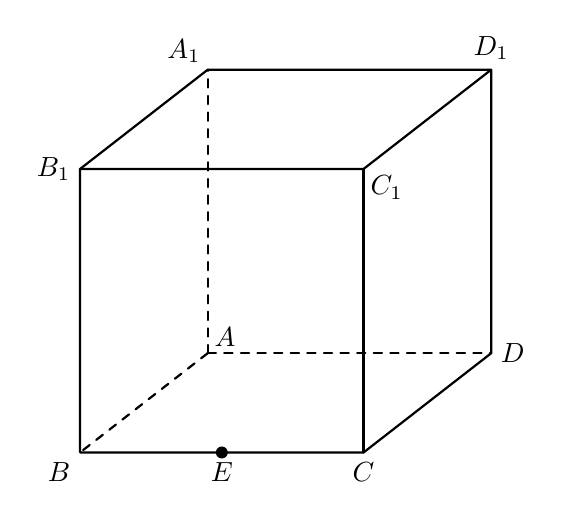
\begin{tikzpicture}[scale=1.8, line join=round, line cap=round, >=stealth]
  % 顶点坐标设定（正方体斜二测标准投影）
  \coordinate (B) at (0, 0);
  \coordinate (C) at (2.0, 0);
  \coordinate (A) at (0.9, 0.7);
  \coordinate (D) at (2.9, 0.7);

  \coordinate (B1) at (0, 2.0);
  \coordinate (C1) at (2.0, 2.0);
  \coordinate (A1) at (0.9, 2.7);
  \coordinate (D1) at (2.9, 2.7);

  % 棱 BC 中点 E
  \coordinate (E) at (1.0, 0);

  % 虚线部分（后侧与内部不可见棱）
  \draw[dashed, thick] (A) -- (B);
  \draw[dashed, thick] (A) -- (D);
  \draw[dashed, thick] (A) -- (A1);

  % 实线部分（外轮廓与可见棱）
  \draw[thick] (B) -- (C) -- (D) -- (D1) -- (A1) -- (B1) -- cycle;
  \draw[thick] (B1) -- (C1) -- (D1);
  \draw[thick] (C) -- (C1);

  % 关键点标记
  \fill (E) circle (1.2pt);

  % 顶点标注
  \node[below left] at (B) {$B$};
  \node[below] at (C) {$C$};
  \node[right] at (D) {$D$};
  \node[above right=-1pt] at (A) {$A$};

  \node[left] at (B1) {$B_1$};
  \node[below right=-1pt] at (C1) {$C_1$};
  \node[above] at (D1) {$D_1$};
  \node[above left=-1pt] at (A1) {$A_1$};

  \node[below] at (E) {$E$};
\end{tikzpicture}
\end{center}
\nopagebreak[4]
\Needspace{0.4\textheight}
\end{question}
\begin{question}
\gkti{19}如图，在 $\mathrm{Rt}\triangle ABC$ 中，已知 $BC = a$，若长为 $2a$ 的线段 $PQ$ 以点 $A$ 为中点，问 $\vec{PQ}$ 与 $\vec{BC}$ 的夹角 $\theta$ 取何值时 $\vec{BP} \cdot \vec{CQ}$ 的值最大？并求出这个最大值．
\nopagebreak[4]
\begin{center}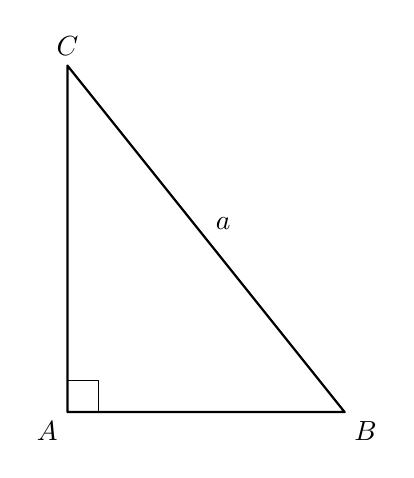
\begin{tikzpicture}[scale=2.2, line join=round, line cap=round]
  \coordinate (A) at (0, 0);
  \coordinate (B) at (1.6, 0);
  \coordinate (C) at (0, 2.0);

  % 绘制直角三角形
  \draw[thick] (A) -- (B) -- (C) -- cycle;

  % 直角标记
  \draw[thin] (0, 0.18) -- (0.18, 0.18) -- (0.18, 0);

  % 顶点与边长标注
  \node[below left] at (A) {$A$};
  \node[below right] at (B) {$B$};
  \node[above] at (C) {$C$};
  \node[above right] at (0.8, 1.0) {$a$};
\end{tikzpicture}
\end{center}
\nopagebreak[4]
\end{question}
\begin{question}
\gkti{20}直线 $l: y = kx + 1$ 与双曲线 $C: 2x^2 - y^2 = 1$ 的右支交于不同的两点 $A$、$B$．

（1）求实数 $k$ 的取值范围；

（2）是否存在实数 $k$，使得以线段 $AB$ 为直径的圆经过双曲线 $C$ 的右焦点 $F$？若存在，求出 $k$ 的值．若不存在，说明理由．

\end{question}
\begin{question}
\gkti{21}某突发事件，在不采取任何预防措施的情况下发生的概率为 $0.3$；一旦发生，将造成 $400$ 万元的损失．现有甲、乙两种相互独立的预防措施可供采用．单独采用甲、乙预防措施所需的费用分别为 $45$ 万元和 $30$ 万元，采用相应预防措施后此突发事件不发生的概率分别是 $0.9$ 和 $0.85$．若预防方案允许甲、乙两种预防措施单独采用、联合采用或不采用，请确定预防方案使总费用最少．

注：总费用 = 采取预防措施的费用 + 发生突发事件损失的期望值．

\end{question}
\begin{question}
\gkti{22}已知 $a > 0$，数列 $\{a_n\}$ 满足 $a_1 = a$，$a_{n+1} = a + \dfrac{1}{a_n}$，$n = 1, 2, \cdots$．

（1）已知数列 $\{a_n\}$ 极限存在且大于零，求 $A = \lim_{n\to\infty} a_n$（将 $A$ 用 $a$ 表示）；

（2）设 $b_n = a_n - A$，$n = 1, 2, \cdots$，证明：$b_{n+1} = -\dfrac{b_n}{A(b_n + A)}$；

（3）若 $|b_n| \leqslant \dfrac{1}{2^n}$ 对 $n = 1, 2, \cdots$ 都成立，求 $a$ 的取值范围．

\end{question}